\documentclass[11pt, oneside]{article} 
\usepackage[margin=1in]{geometry} \geometry{letterpaper} 
\usepackage{setspace}
\usepackage[font=singlespacing,labelfont=bf]{caption}
\usepackage{indentfirst}
\usepackage{float}
\usepackage{booktabs}
\usepackage{amsmath, gensymb}
\usepackage{url}

\usepackage{graphicx}
\makeatletter
\def\maxwidth{0.6\columnwidth}
\makeatother
\let\Oldincludegraphics\includegraphics
\renewcommand{\includegraphics}[1]{\Oldincludegraphics[width=\maxwidth]{#1}}

\title{Markdown To Report\\\vspace{0.5em}{\large A collection of scripts to generate LaTeX formatted PDFs}}
\author{Kai Wells}
\date{}

\hyphenpenalty=100000

\begin{document}

\pagenumbering{gobble}
\maketitle
\begin{table}[H]
\centering
\begin{tabular}{l}
Github Example\\
Due: April 7, 2015\\
Received: April 7, 2015\\
\end{tabular}
\end{table}
\begin{noindent}
\textbf{Normally this is a brief summary of the important results found in an experiment. This is just an example.}
\end{noindent}

\newpage
\doublespacing
\pagenumbering{arabic}

\section{Introduction}

This is a brief example of what this collection of scripts does. The metadata above is used to generate the title page of the report.

\begin{figure}[H]
\centering
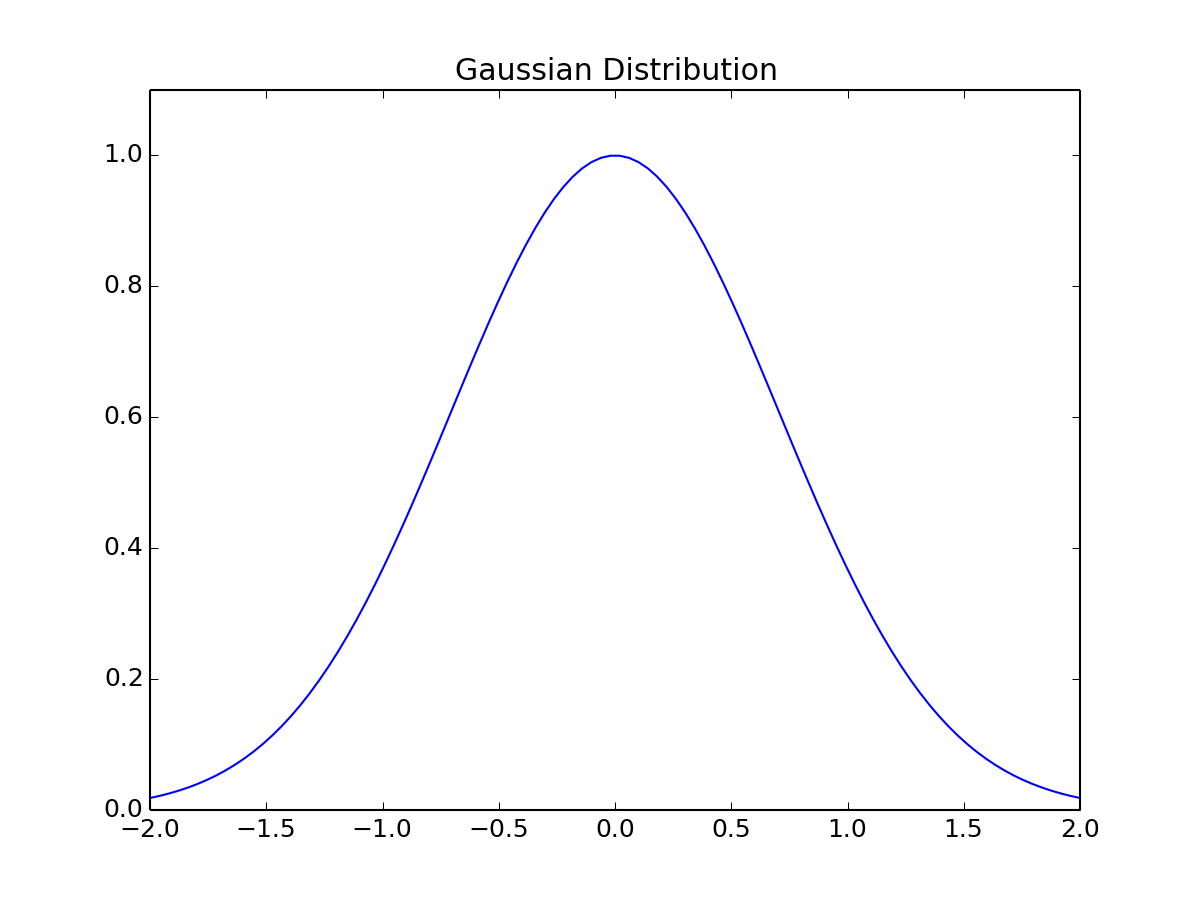
\includegraphics{graph.png}
\caption{Images with captions are defined like so.}
\label{fig:labels-are-required}
\end{figure}

\begin{table}[H]
\caption{This is an example table.}
\centering
\begin{tabular}{|l|ccr|}
\hline
a & b & c & d\\
\hline
1 & 2 & 3 & 4\\
\hline
\end{tabular}
\label{table:labels-are-required-too}
\end{table}

Figure and table labels are required and must appear in [square brackets] below the object they are labeling.

\begin{equation}
E = m c^2
\label{eq:optional}
\end{equation}

Equations have to be entered in standard LaTeX format. As do \emph{italicized} and \textbf{bolded} passages. I'll work on that in the future.

Careful of typos! The makefile will hang if it encounters a LaTeX error while converting to PDF.

\end{document}
